\documentclass[11pt,a4paper]{article}
\usepackage[utf8]{inputenc}
\usepackage[T1]{fontenc}
\usepackage[margin=2.2cm]{geometry}
\usepackage{amsmath,amssymb}
\usepackage{graphicx}
\usepackage{booktabs,array,multirow}
\usepackage{tikz}
\usetikzlibrary{arrows.meta,positioning,calc}
\renewcommand{\figurename}{Figura}
\renewcommand{\tablename}{Tabla}
\usepackage{listings}
\usepackage{xcolor}
\usepackage{enumitem}
\usepackage{fancyhdr}
\usepackage[hidelinks]{hyperref}

\definecolor{azulpucp}{RGB}{0,60,120}
\definecolor{grisc}{RGB}{245,245,245}
\definecolor{verdecod}{RGB}{20,110,20}

\lstset{
  language=Matlab, basicstyle=\ttfamily\small, numbers=left,
  numberstyle=\tiny\color{gray}, numbersep=8pt, frame=single,
  framerule=0.3pt, backgroundcolor=\color{grisc},
  commentstyle=\color{verdecod}, keywordstyle=\color{azulpucp}\bfseries,
  showstringspaces=false, breaklines=true, columns=flexible
}

% Derivada parcial simple y derivada parcial total (notacion del curso: barras)
\newcommand{\pd}[2]{\frac{\partial #1}{\partial #2}}
\newcommand{\td}[2]{\frac{\overline{\partial #1}}{\overline{\partial #2}}}
\newcommand{\grados}{^{\circ}}

\pagestyle{fancy}
\fancyhf{}
\fancyhead[L]{\small Examen Final 2025-1 — Desarrollo}
\fancyhead[R]{\small Redes Neuronales Aplicadas al Control}
\fancyfoot[C]{\small\thepage}

\setlength{\parskip}{4pt}
\setlength{\parindent}{0pt}

\newenvironment{enunciado}
{\begin{quote}\small\itshape\color{azulpucp}}
{\end{quote}}

\begin{document}

\begin{center}
{\large\bfseries Pontificia Universidad Católica del Perú}\\[2pt]
{\bfseries Maestría en Ingeniería de Control y Automatización}\\[8pt]
{\Large\bfseries Examen Final 2025-1 — Desarrollo}\\[4pt]
{\normalsize Curso: Redes Neuronales Aplicadas al Control}\\[2pt]
{\small Guía de estudio elaborada a partir de las notas del curso (Clases 7, 9, 10, 11, 12 y 13)}
\end{center}

\vspace{4pt}
\hrule
\vspace{10pt}

%=====================================================================
\section*{Pregunta 1 (4 ptos) — Control lineal--difuso del robot truck--tráiler para coordenadas iniciales $y$ alejadas de $y^{*}=0$}

\begin{enunciado}
Se ha diseñado un controlador para un robot móvil tipo truck--tráiler de dos cuerpos articulados basado en la integración de un controlador difuso con un controlador lineal diseñado según el método de linealización por aproximación, para alcanzar la posición deseada $y^{*}=0$, $\theta_2^{*}=0$, $\theta_{12}^{*}=0$, $\delta^{*}=0$. El controlador trabaja bien para valores iniciales de la coordenada $y$ cercanos a $0$. Explicar el proceso de diseño del controlador para que el robot alcance la posición deseada desde coordenadas iniciales $y$ alejadas de $y^{*}=0$.
\end{enunciado}

\subsection*{1.1 Revisión del diseño base (Clase 13)}

\textbf{Paso 1 — Modelo cinemático.} El robot truck--tráiler se modela como dos barras articuladas (truck de longitud $L_1$, tráiler de longitud $L_2$), moviéndose en retroceso a velocidad constante $v$, sin deslizamiento de ruedas. Con $\theta_{12}=\theta_1-\theta_2$ (ángulo truck--tráiler) las ecuaciones de movimiento son:
\begin{align}
\dot{y} &= v\,\cos\theta_{12}\,\sin\theta_2 \\
\dot{\theta}_2 &= -\frac{v}{L_2}\,\sin\theta_{12} \\
\dot{\theta}_{12} &= \frac{v}{L_2}\,\sin\theta_{12} - \frac{v}{L_1}\,\tan\delta
\end{align}
Se define el vector de estado $\mathbf{x}=[\,y\ \ \theta_2\ \ \theta_{12}\,]^{T}$ y la entrada $u=\tan\delta$. La coordenada $x$ \emph{no} se incluye en el estado: como $v$ es constante, al converger a la recta $y=0$ se cumple $\dot x = v$, es decir $x$ se comporta como el tiempo (variable independiente), y la estrategia de control es: \emph{primero} alcanzar la recta $y^{*}=0$ con $\theta_2^{*}=0$, $\theta_{12}^{*}=0$ y \emph{después} avanzar en línea recta hasta la posición final, pasando entre los obstáculos.

\textbf{Paso 2 — Linealización por aproximación.} Alrededor del punto deseado ($y^{*}=0$, $\theta_2^{*}=0$, $\theta_{12}^{*}=0$, $\delta^{*}=0$) se aproxima $\sin\theta\approx\theta$, $\cos\theta\approx 1$:
\begin{equation}
\begin{bmatrix}\dot y\\ \dot\theta_2\\ \dot\theta_{12}\end{bmatrix}
=
\begin{bmatrix}0 & v & 0\\ 0 & 0 & -v/L_2\\ 0 & 0 & v/L_2\end{bmatrix}
\begin{bmatrix}y\\ \theta_2\\ \theta_{12}\end{bmatrix}
+
\begin{bmatrix}0\\ 0\\ -v/L_1\end{bmatrix}\tan\delta
\label{eq:linmodel}
\end{equation}

\textbf{Paso 3 — Controlador lineal.} Para el modelo \eqref{eq:linmodel} se diseña una ley de realimentación completa de estados
\begin{equation}
\tan\delta = -k_1\,y - k_2\,\theta_2 - k_3\,\theta_{12}
\label{eq:leylineal}
\end{equation}
eligiendo $k_1,k_2,k_3$ por asignación de polos (o LQR) de modo que el lazo cerrado lineal sea estable.

\textbf{Paso 4 — Integración difusa en $\theta_{12}$ (evitar jack--knife).} La ley \eqref{eq:leylineal} sólo es válida cerca de $\theta_{12}=0$; para $\theta_{12}$ cercanos a $\pm 90\grados$ (posición jack--knife) no garantiza estabilidad. El rango de $\theta_{12}$ se particiona en tres valores lingüísticos (\emph{Negative Big}, \emph{Zero}, \emph{Positive Big}), se diseña un controlador simple para cada partición y se integran mediante lógica difusa. De la ecuación (3) se observa la relación inversa entre $\dot\theta_{12}$ y $\tan\delta$, lo que da las reglas:
\begin{center}
\begin{tabular}{l}
\textbf{IF } $\theta_{12}$ = Positive Big \textbf{ THEN } $\delta=\delta_{\max}$ (positivo)\\
\textbf{IF } $\theta_{12}$ = Zero \textbf{ THEN } $\delta$ = ley lineal \eqref{eq:leylineal}\\
\textbf{IF } $\theta_{12}$ = Negative Big \textbf{ THEN } $\delta=\delta_{\min}$ (negativo)
\end{tabular}
\end{center}
La salida del controlador integrado es la \textbf{suma ponderada} de las salidas de los tres controladores, con pesos dados por los valores de pertenencia de $\theta_{12}$ a cada partición:
\begin{equation}
\delta = \frac{\mu_{NB}(\theta_{12})\,\delta_{\min} + \mu_{ZE}(\theta_{12})\,\delta_{lin} + \mu_{PB}(\theta_{12})\,\delta_{\max}}
{\mu_{NB}(\theta_{12}) + \mu_{ZE}(\theta_{12}) + \mu_{PB}(\theta_{12})}
\label{eq:sumapond}
\end{equation}

\begin{figure}[h]
\centering
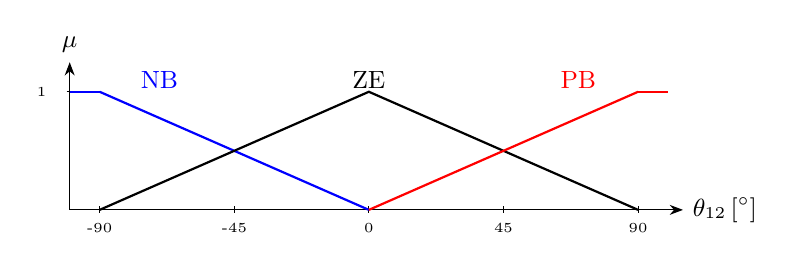
\begin{tikzpicture}[xscale=0.038,yscale=1.5]
% ejes
\draw[-{Stealth}] (-100,0) -- (105,0) node[right] {\small $\theta_{12}\,[\grados]$};
\draw[-{Stealth}] (-100,0) -- (-100,1.25) node[above] {\small $\mu$};
\foreach \x in {-90,-45,0,45,90} \draw (\x,0.03) -- (\x,-0.03) node[below] {\tiny \x};
\draw (-101,1) -- (-99,1) node[left=6pt] {\tiny 1};
% NB: 1 en -90, baja a 0 en 0
\draw[thick,blue] (-90,1) -- (0,0);
\draw[thick,blue] (-100,1) -- (-90,1);
\node[blue] at (-70,1.1) {\small NB};
% ZE triangulo pico 0
\draw[thick,black] (-90,0) -- (0,1) -- (90,0);
\node at (0,1.1) {\small ZE};
% PB
\draw[thick,red] (0,0) -- (90,1);
\draw[thick,red] (90,1) -- (100,1);
\node[red] at (70,1.1) {\small PB};
\end{tikzpicture}
\caption{Particiones y funciones de pertenencia del ángulo truck--tráiler $\theta_{12}$ (traslape entre particiones contiguas; ancho de la partición ZE ajustable: una ZE más ancha da convergencia más rápida a costa de $\theta_{12}$ y $\delta$ mayores).}
\end{figure}

\subsection*{1.2 ¿Por qué el diseño base sólo funciona con $y$ cercano a 0?}

\begin{itemize}[itemsep=2pt]
\item La linealización $\sin\theta_2\approx\theta_2$ sólo vale para $\theta_2$ pequeños. Pero para acercarse a la recta $y=0$ desde un $y$ lejano, el robot \emph{necesita} inclinaciones $\theta_2$ grandes (debe ``apuntar'' hacia la recta): la maniobra correcta sale de la región de validez del modelo linealizado.
\item Con $y$ grande, el término $-k_1 y$ de la ley \eqref{eq:leylineal} produce valores de $\tan\delta$ enormes: el timón se satura ($\delta\in[-30\grados,30\grados]$), el lazo deja de comportarse como el lazo lineal diseñado y pueden inducirse posiciones jack--knife.
\item La ley lineal intenta lograr \emph{simultáneamente} $y\to 0$ y $\theta_2\to 0$, lo que es geométricamente imposible desde lejos: primero hay que reorientar el vehículo hacia la recta y sólo al final alinear $\theta_2\to 0$.
\end{itemize}

\subsection*{1.3 Proceso de diseño extendido para $y$ alejados de $y^{*}=0$}

La idea del curso se mantiene: \emph{diseñar controladores simples válidos en regiones (particiones) del espacio de estado e integrarlos mediante lógica difusa como suma ponderada por las pertenencias}. Ahora la partición se hace también sobre la coordenada $y$.

\textbf{Paso 1 — Consigna intermedia de orientación.} Cuando $|y|$ es grande, el objetivo instantáneo ya no es $\theta_2^{*}=0$ sino \emph{aproximarse a la recta} con un ángulo de aproximación grande. Se define la consigna de inclinación deseada del tráiler como función saturada de $y$:
\begin{equation}
\theta_2^{*}(y) = -\bar{\theta}_2\,\mathrm{sat}\!\left(\frac{y}{y_a}\right),
\qquad
\mathrm{sat}(s)=\begin{cases} 1 & s>1\\ s & |s|\le 1\\ -1 & s<-1\end{cases}
\label{eq:consigna}
\end{equation}
donde $\bar{\theta}_2$ es el ángulo máximo de aproximación (por ejemplo $60\grados$--$90\grados$, con el signo elegido según el sentido de avance $v$ de modo que el movimiento reduzca $|y|$) y $y_a$ define el ancho de la zona de transición. Lejos de la recta el robot se aproxima con inclinación $\pm\bar\theta_2$ casi constante; cerca de la recta la consigna tiende suavemente a $0$.

\textbf{Paso 2 — Ley lineal con consignas variables.} Se usa la versión de la ley lineal para posiciones deseadas arbitrarias (ecuación (13) del paper de la Clase 13), con $\theta_{12}^{*}=0$ y $\delta^{*}=0$:
\begin{equation}
\tan\delta = -k_2\,\bigl(\theta_2-\theta_2^{*}(y)\bigr) - k_3\,\theta_{12}
\label{eq:leyext}
\end{equation}
\textbf{Verificación de consistencia:} cerca de la recta, $\mathrm{sat}(y/y_a)\approx y/y_a$ y la ley \eqref{eq:leyext} se reduce a
$\tan\delta \approx -(k_2\bar\theta_2/y_a)\,y - k_2\,\theta_2 - k_3\,\theta_{12}$,
es decir, se \emph{recupera exactamente} la ley lineal original \eqref{eq:leylineal} con $k_1\equiv k_2\bar\theta_2/y_a$. La transición es suave, sin conmutaciones bruscas.

\textbf{Paso 3 — Formulación difusa equivalente.} Alternativamente (y de forma totalmente coherente con la metodología del curso), se particiona $y$ en tres valores lingüísticos $\{NG,\,ZE,\,PG\}$ y se asigna un controlador simple a cada partición:
\begin{center}
\begin{tabular}{l}
\textbf{IF } $y$ = PG (muy arriba) \textbf{ THEN } $\delta$ = ley \eqref{eq:leyext} con $\theta_2^{*}=-\bar\theta_2$ (bajar hacia la recta)\\
\textbf{IF } $y$ = ZE (cerca de la recta) \textbf{ THEN } $\delta$ = ley lineal original \eqref{eq:leylineal}\\
\textbf{IF } $y$ = NG (muy abajo) \textbf{ THEN } $\delta$ = ley \eqref{eq:leyext} con $\theta_2^{*}=+\bar\theta_2$ (subir hacia la recta)
\end{tabular}
\end{center}
y la salida total es la suma ponderada por las pertenencias $\mu_{NG}(y),\mu_{ZE}(y),\mu_{PG}(y)$, igual que en \eqref{eq:sumapond}.

\textbf{Paso 4 — Prioridad anti jack--knife.} Las reglas del diseño base sobre $\theta_{12}$ (partición $NB/ZE/PB$) se mantienen y \emph{dominan} sobre las reglas en $y$: si $\theta_{12}$ entra en $PB$ o $NB$, la salida se satura en $\delta_{\max}$ o $\delta_{\min}$ para llevar $\theta_{12}$ hacia cero, independientemente de lo que pidan las reglas de posicionamiento. Esto garantiza que las maniobras amplias requeridas desde $y$ lejano no produzcan jack--knife.

\textbf{Paso 5 — Verificación por simulación.} Se simula el lazo cerrado desde múltiples posiciones iniciales (distintos $y_0$, $\theta_{2,0}$, $\theta_{12,0}$), verificando: (i) convergencia asintótica a $y^{*}=0$, $\theta_2^{*}=0$, $\theta_{12}^{*}=0$; (ii) $\delta$ acotado en $[\delta_{\min},\delta_{\max}]=[-30\grados,+30\grados]$; (iii) $|\theta_{12}|$ lejos de $90\grados$ en todo momento; (iv) no colisión con los obstáculos. Con los resultados se ajustan $\bar\theta_2$, $y_a$ y el ancho de las particiones.

\begin{figure}[h]
\centering
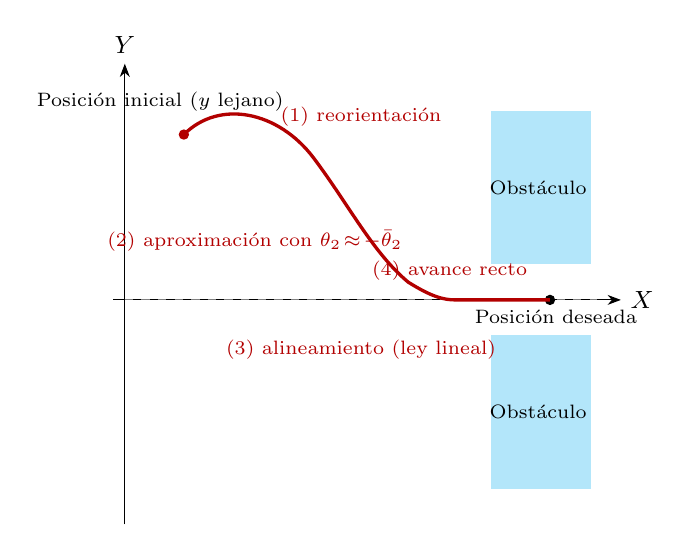
\begin{tikzpicture}[scale=0.075]
% Ejes
\draw[-{Stealth}] (0,-38) -- (0,40) node[above] {\small $Y$};
\draw[-{Stealth}] (-2,0) -- (84,0) node[right] {\small $X$};
\draw[dashed,gray] (0,0) -- (80,0);
% Obstaculos
\fill[cyan!30] (62,6) rectangle (79,32);
\fill[cyan!30] (62,-32) rectangle (79,-6);
\node at (70,19) {\scriptsize Obstáculo};
\node at (70,-19) {\scriptsize Obstáculo};
% Posicion deseada
\node at (73,-2.8) {\scriptsize Posición deseada};
\fill (72,0) circle (25pt);
% Trayectoria
\draw[very thick,red!70!black]
 (10,28) .. controls (16,34) and (26,32) .. (32,24)
         .. controls (38,16) and (42,8) .. (48,3)
         .. controls (52,0.5) and (54,0) .. (56,0) -- (72,0);
\fill[red!70!black] (10,28) circle (25pt);
\node at (6,33.5) {\scriptsize Posición inicial ($y$ lejano)};
% Fases
\node[red!70!black] at (40,31) {\scriptsize (1) reorientación};
\node[red!70!black] at (22,10) {\scriptsize (2) aproximación con $\theta_2\!\approx\!-\bar\theta_2$};
\node[red!70!black] at (40,-8.5) {\scriptsize (3) alineamiento (ley lineal)};
\node[red!70!black] at (55,5) {\scriptsize (4) avance recto};
\end{tikzpicture}
\hspace{8mm}
\begin{tikzpicture}[xscale=0.055,yscale=0.022]
\draw[-{Stealth}] (-45,0) -- (48,0) node[right] {\small $y$};
\draw[-{Stealth}] (0,-95) -- (0,95) node[above] {\small $\theta_2^{*}(y)$};
\draw[very thick,blue] (-45,75) -- (-15,75) -- (15,-75) -- (45,-75);
\draw[dashed] (15,0) -- (15,-75) -- (0,-75);
\node[below] at (17,-1) {\tiny $y_a$};
\node[left] at (0,-75) {\tiny $-\bar\theta_2$};
\node[left] at (0,75) {\tiny $+\bar\theta_2$};
\end{tikzpicture}
\caption{Izquierda: fases de la trayectoria con el controlador extendido. Derecha: consigna de orientación saturada $\theta_2^{*}(y)$; en la zona $|y|<y_a$ se recupera la ley lineal original.}
\end{figure}

%=====================================================================
\clearpage
\section*{Pregunta 2 (4 ptos) — Controlador difuso para el ángulo $\theta_2$ de un motor CC con reductor}

\begin{enunciado}
Diseñar un sistema difuso para controlar el ángulo de giro $\theta_2$ del motor CC con reductor. Sistema: $\dot{\mathbf x}=A\mathbf x+B u$, $\mathbf x=[\,\theta_2\ \dot\theta_2\ i\,]^T$. Voltaje $\in[-24,24]$ V; $\theta_2\in[-45\grados,45\grados]$; $\dot\theta_2\in[-10,10]\ \grados/s$. Tres particiones para las entradas y tres para la salida. Voltaje positivo $\Rightarrow$ giro antihorario (positivo). Objetivo: $\theta_2\to 0$ desde cualquier posición inicial. Explicar todo el proceso de diseño, el cálculo de la salida para valores arbitrarios de $\theta_2$ y $\dot\theta_2$, y representar el controlador mediante una red neuro--difusa.
\end{enunciado}

\subsection*{2.1 Entradas y salida del controlador (proceso de diseño, Clase 11)}

Aunque el sistema tiene tres variables de estado, el controlador difuso usa como entradas las dos variables dominantes del objetivo de control: la \textbf{posición angular} $\theta_2$ y la \textbf{velocidad angular} $\dot\theta_2$ (la corriente $i$ tiene dinámica eléctrica rápida y no se necesita como entrada del controlador). La velocidad es indispensable: sin ella el controlador no puede ``frenar'' a tiempo y el eje oscilaría alrededor de $\theta_2^{*}=0$. La salida es el voltaje $V$ aplicado al motor.
\[
\theta_2^{*}=0,\qquad \dot\theta_2^{*}=0,\qquad V^{*}=0
\]
Los valores deseados quedan en el \textbf{punto medio} de cada rango, como exige la metodología del curso.

\subsection*{2.2 Rangos de variación}

\[
-45\grados \le \theta_2 \le 45\grados,\qquad
-10\ \grados/s \le \dot\theta_2 \le 10\ \grados/s,\qquad
-24\ \mathrm{V} \le V \le 24\ \mathrm{V}
\]
(El rango de $\dot\theta_2$ se determina experimentalmente aplicando el voltaje máximo y midiendo la velocidad alcanzada; si fuera necesario se da un margen adicional del 20--30\%. Al voltaje también podría dársele margen, p.\,ej.\ $\pm 30$ V, para garantizar que la defuzzificación pueda alcanzar el voltaje máximo físico; aquí mantenemos $\pm 24$ V del enunciado.)

\subsection*{2.3 Particiones, valores lingüísticos y funciones de pertenencia}

Cada variable se particiona en un número \textbf{impar} (3) de particiones \textbf{simétricas}, con \textbf{traslape} entre particiones contiguas y suma de pertenencias igual a 1:
\[
\theta_2:\ \{NE,\,ZE,\,PO\},\qquad \dot\theta_2:\ \{NE,\,ZE,\,PO\},\qquad V:\ \{NE,\,ZE,\,PO\}
\]

\begin{figure}[h]
\centering
% MF theta2
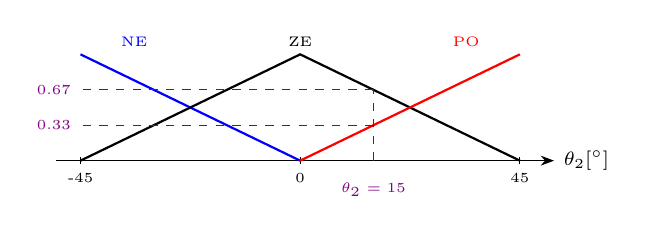
\begin{tikzpicture}[xscale=0.062,yscale=1.35]
\draw[-{Stealth}] (-50,0) -- (52,0) node[right] {\scriptsize $\theta_2[\grados]$};
\foreach \x in {-45,0,45} \draw (\x,0.03) -- (\x,-0.03) node[below] {\tiny \x};
\draw[thick,blue] (-45,1) -- (0,0); \node[blue] at (-34,1.12) {\tiny NE};
\draw[thick] (-45,0) -- (0,1) -- (45,0); \node at (0,1.12) {\tiny ZE};
\draw[thick,red] (0,0) -- (45,1); \node[red] at (34,1.12) {\tiny PO};
% marca en 15
\draw[dashed,violet] (15,0) -- (15,0.6667);
\draw[dashed,violet] (15,0.6667) -- (-45,0.6667) node[left] {\tiny 0.67};
\draw[dashed,violet] (15,0.3333) -- (-45,0.3333) node[left] {\tiny 0.33};
\node[violet,below] at (15,-0.12) {\tiny $\theta_2=15$};
\end{tikzpicture}\hfill
% MF dtheta2
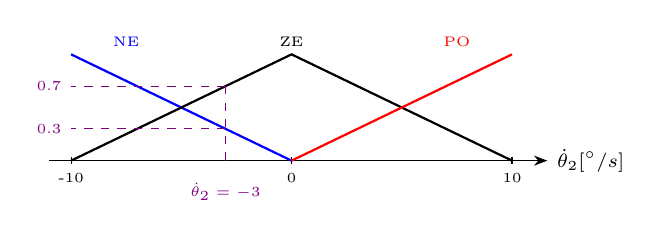
\begin{tikzpicture}[xscale=0.28,yscale=1.35]
\draw[-{Stealth}] (-11,0) -- (11.6,0) node[right] {\scriptsize $\dot\theta_2[\grados/s]$};
\foreach \x in {-10,0,10} \draw (\x,0.03) -- (\x,-0.03) node[below] {\tiny \x};
\draw[thick,blue] (-10,1) -- (0,0); \node[blue] at (-7.5,1.12) {\tiny NE};
\draw[thick] (-10,0) -- (0,1) -- (10,0); \node at (0,1.12) {\tiny ZE};
\draw[thick,red] (0,0) -- (10,1); \node[red] at (7.5,1.12) {\tiny PO};
\draw[dashed,violet] (-3,0) -- (-3,0.7);
\draw[dashed,violet] (-3,0.7) -- (-10,0.7) node[left] {\tiny 0.7};
\draw[dashed,violet] (-3,0.3) -- (-10,0.3) node[left] {\tiny 0.3};
\node[violet,below] at (-3,-0.12) {\tiny $\dot\theta_2=-3$};
\end{tikzpicture}\hfill
% MF V
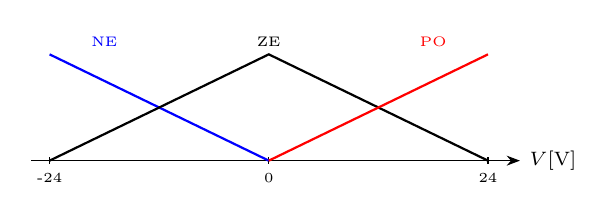
\begin{tikzpicture}[xscale=0.116,yscale=1.35]
\draw[-{Stealth}] (-26,0) -- (27.5,0) node[right] {\scriptsize $V$[V]};
\foreach \x in {-24,0,24} \draw (\x,0.03) -- (\x,-0.03) node[below] {\tiny \x};
\draw[thick,blue] (-24,1) -- (0,0); \node[blue] at (-18,1.12) {\tiny NE};
\draw[thick] (-24,0) -- (0,1) -- (24,0); \node at (0,1.12) {\tiny ZE};
\draw[thick,red] (0,0) -- (24,1); \node[red] at (18,1.12) {\tiny PO};
\end{tikzpicture}
\caption{Funciones de pertenencia triangulares de $\theta_2$, $\dot\theta_2$ y $V$ (traslape, simetría, suma $=1$), con la fuzzificación del ejemplo $\theta_2=+15\grados$, $\dot\theta_2=-3\ \grados/s$.}
\label{fig:mfs}
\end{figure}

\subsection*{2.4 Base de reglas (9 reglas)}

Física del sistema: voltaje positivo $\Rightarrow$ el eje 2 gira en sentido antihorario ($\dot\theta_2$ aumenta). Para llevar $\theta_2\to 0$: si $\theta_2>0$ se necesita velocidad negativa (voltaje negativo); si $\theta_2<0$, voltaje positivo; y la velocidad se usa para frenar (amortiguar) al acercarse. Para cada combinación de valores lingüísticos de las entradas se formula una regla con la experiencia de un operador humano ($3\times 3=9$ reglas):

\begin{table}[h]
\centering
\begin{tabular}{c|ccc}
\toprule
\multirow{2}{*}{$\theta_2$} & \multicolumn{3}{c}{$\dot\theta_2$}\\
 & NE & ZE & PO\\
\midrule
NE & PO & PO & ZE\\
ZE & PO & ZE & NE\\
PO & ZE & NE & NE\\
\bottomrule
\end{tabular}
\caption{Base de reglas: valor lingüístico del voltaje $V$.}
\end{table}

Justificación de reglas representativas:
\begin{itemize}[itemsep=1pt]
\item \textbf{IF} $\theta_2=PO$ \textbf{AND} $\dot\theta_2=PO$ \textbf{THEN} $V=NE$: el eje está adelantado \emph{y alejándose}; hay que frenar y regresarlo con voltaje negativo.
\item \textbf{IF} $\theta_2=PO$ \textbf{AND} $\dot\theta_2=NE$ \textbf{THEN} $V=ZE$: el eje está adelantado pero \emph{ya regresa} solo; no se aplica voltaje para no sobrepasar el objetivo.
\item \textbf{IF} $\theta_2=ZE$ \textbf{AND} $\dot\theta_2=PO$ \textbf{THEN} $V=NE$: en el objetivo pero moviéndose: frenar.
\item \textbf{IF} $\theta_2=ZE$ \textbf{AND} $\dot\theta_2=ZE$ \textbf{THEN} $V=ZE$: objetivo logrado, no actuar.
\end{itemize}
(Las reglas con $\theta_2=NE$ son simétricas.) La base de reglas es antisimétrica respecto al centro, como corresponde a un problema de estabilización simétrico: es un ``PD difuso''.

\subsection*{2.5 Cálculo de la salida: inferencia MIN--MAX (Mamdani) con ejemplo numérico}

Valores arbitrarios elegidos: $\boxed{\theta_2=+15\grados,\quad \dot\theta_2=-3\ \grados/s}$

\textbf{(i) Fuzzificación} (ver Figura \ref{fig:mfs}):
\[
\mu_{ZE}(\theta_2)=1-\tfrac{15}{45}=0.67,\quad
\mu_{PO}(\theta_2)=\tfrac{15}{45}=0.33,\qquad
\mu_{NE}(\dot\theta_2)=\tfrac{3}{10}=0.30,\quad
\mu_{ZE}(\dot\theta_2)=1-\tfrac{3}{10}=0.70
\]
(las demás pertenencias son cero).

\textbf{(ii) Reglas activas y operador AND = mínimo} (se activan $2\times 2=4$ reglas):
\begin{center}
\begin{tabular}{llll}
\toprule
Regla & Antecedente & Consecuente & Grado de activación\\
\midrule
R1 & $\theta_2=ZE$ \textbf{AND} $\dot\theta_2=NE$ & $V=PO$ & $\min(0.67,\,0.30)=0.30$\\
R2 & $\theta_2=ZE$ \textbf{AND} $\dot\theta_2=ZE$ & $V=ZE$ & $\min(0.67,\,0.70)=0.67$\\
R3 & $\theta_2=PO$ \textbf{AND} $\dot\theta_2=NE$ & $V=ZE$ & $\min(0.33,\,0.30)=0.30$\\
R4 & $\theta_2=PO$ \textbf{AND} $\dot\theta_2=ZE$ & $V=NE$ & $\min(0.33,\,0.70)=0.33$\\
\bottomrule
\end{tabular}
\end{center}

\textbf{(iii) Agregación (máximo por consecuente):} la partición $PO$ queda recortada a $0.30$; la partición $ZE$ a $\max(0.67,\,0.30)=0.67$; y la partición $NE$ a $0.33$.

\textbf{(iv) Defuzzificación.}

\emph{Método de Sugeno} (valores representativos $NE=-24$, $ZE=0$, $PO=+24$):
\[
V=\frac{0.30(+24)+0.67(0)+0.30(0)+0.33(-24)}{0.30+0.67+0.30+0.33}
=\frac{7.2-8.0}{1.60}
=\boxed{-0.5\ \mathrm{V}}
\]

\emph{Método del centro de gravedad (Mandami)}: se toma el centroide del área agregada (triángulos recortados, envolvente por máximo), obteniéndose $V\approx -0.21$ V.

\textbf{Interpretación física:} el eje está adelantado ($+15\grados$) pero ya está regresando ($-3\ \grados/s$); el controlador aplica un voltaje pequeño y negativo: deja que el eje regrese casi solo, empujándolo levemente hacia $\theta_2=0$ sin provocar sobrepaso. El resultado es coherente.

\begin{figure}[h]
\centering
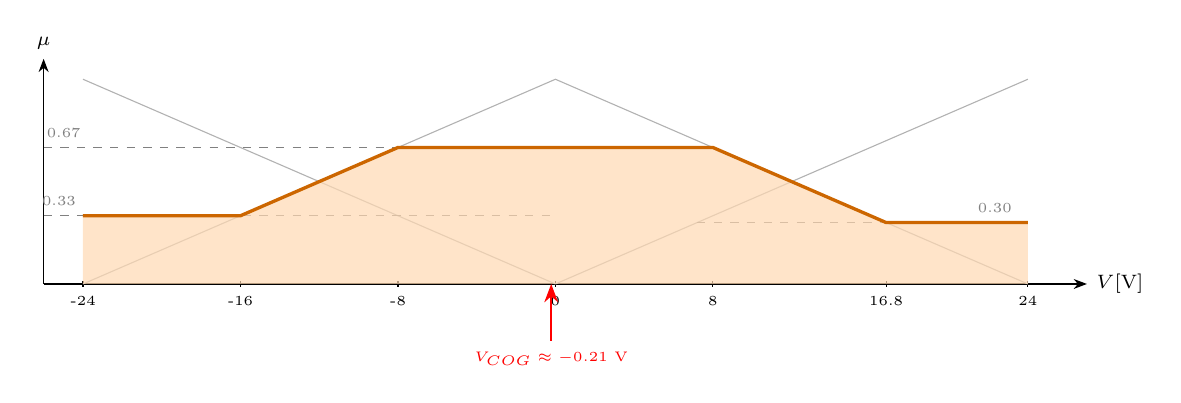
\begin{tikzpicture}[xscale=0.25,yscale=2.6]
\draw[-{Stealth}] (-26,0) -- (27,0) node[right] {\scriptsize $V$[V]};
\draw[-{Stealth}] (-26,0) -- (-26,1.1) node[above] {\scriptsize $\mu$};
\foreach \x in {-24,-16,-8,0,8,16.8,24} \draw (\x,0.014) -- (\x,-0.014) node[below] {\tiny \x};
% MFs claras
\draw[gray!60] (-24,1) -- (0,0); \draw[gray!60] (-24,0) -- (0,1) -- (24,0); \draw[gray!60] (0,0) -- (24,1);
% niveles de recorte
\draw[dashed,gray] (-26,0.3333) -- (0,0.3333) node[pos=0.03,above] {\tiny 0.33};
\draw[dashed,gray] (-26,0.6667) -- (8,0.6667) node[pos=0.03,above] {\tiny 0.67};
\draw[dashed,gray] (7.2,0.30) -- (24,0.30) node[pos=0.9,above] {\tiny 0.30};
% envolvente agregada
\fill[orange!30,opacity=0.7] (-24,0) -- (-24,0.3333) -- (-16,0.3333) -- (-8,0.6667) -- (8,0.6667) -- (16.8,0.30) -- (24,0.30) -- (24,0) -- cycle;
\draw[very thick,orange!80!black] (-24,0.3333) -- (-16,0.3333) -- (-8,0.6667) -- (8,0.6667) -- (16.8,0.30) -- (24,0.30);
% centroides
\draw[{Stealth}-,thick,red] (-0.215,0) -- (-0.215,-0.28) node[below] {\tiny $V_{COG}\approx-0.21$ V};
\end{tikzpicture}
\caption{Salidas recortadas por los grados de activación, área agregada (máximo) y centro de gravedad.}
\end{figure}

\subsection*{2.6 Representación mediante una red neuro--difusa (Clase 12, red Tipo 1)}

El controlador difuso se representa con una red neuronal cuya estructura reproduce las etapas de la lógica difusa:

\begin{itemize}[itemsep=1pt]
\item \textbf{Capa 1 (entradas):} valores numéricos $\theta_2$ y $\dot\theta_2$.
\item \textbf{Capa 2 (fuzzificación):} 6 neuronas, una por función de pertenencia ($NE,ZE,PO$ de cada entrada). Cada neurona implementa una función de pertenencia parametrizada (p.\,ej.\ triangular o sigmoidea con \emph{centro} $c$ y \emph{pendiente} $a$).
\item \textbf{Capa 3 (reglas):} 9 neuronas; la regla $R_i$ calcula su grado de activación $\mu_i$ con el operador AND implementado como \textbf{producto} (o mínimo) de las dos pertenencias de su antecedente.
\item \textbf{Capa 4 (normalización):} calcula el factor $\Sigma=\sum_i\mu_i$ y normaliza $\bar\mu_i=\mu_i/\Sigma$.
\item \textbf{Capa 5 (defuzzificación / salida):} suma ponderada con los valores representativos $f_i$ del consecuente de cada regla ($f_i\in\{-24,0,+24\}$ V según la base de reglas):
\[
V=\frac{\sum_{i=1}^{9}\mu_i\,f_i}{\sum_{i=1}^{9}\mu_i}=\sum_{i=1}^{9}\bar\mu_i\,f_i
\]
\end{itemize}

\begin{figure}[h]
\centering
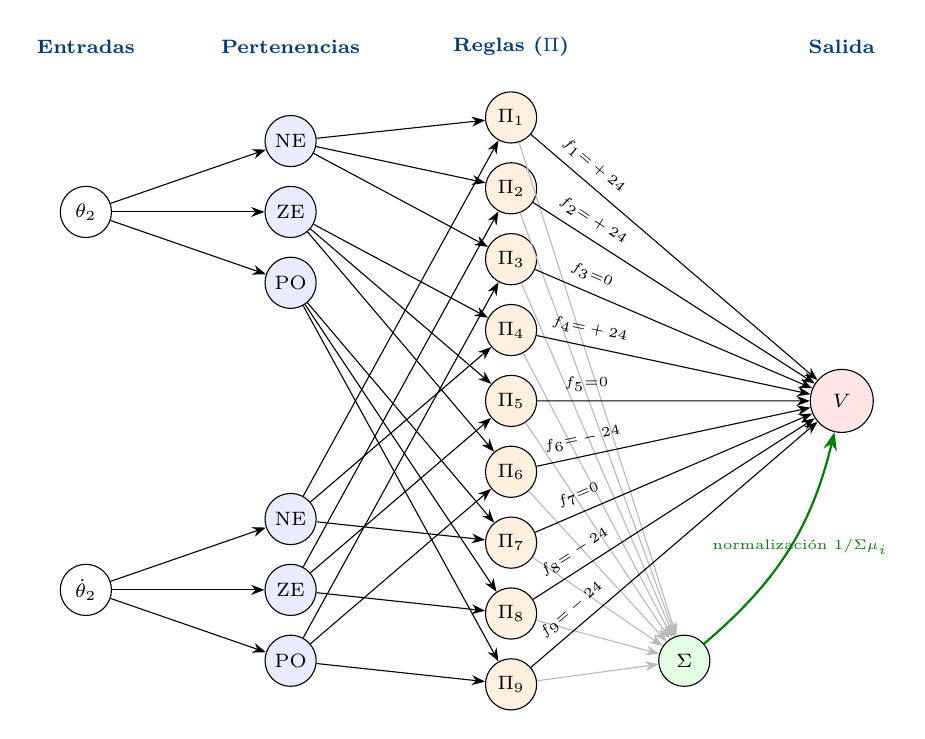
\begin{tikzpicture}[
  neuron/.style={circle,draw,minimum size=6.5mm,inner sep=0pt,font=\scriptsize},
  capT/.style={font=\scriptsize\bfseries,azulpucp}
]
% entradas
\node[neuron] (i1) at (0,6.9) {$\theta_2$};
\node[neuron] (i2) at (0,2.1) {$\dot\theta_2$};
% MFs
\foreach \n/\y/\l in {m1/7.8/NE, m2/6.9/ZE, m3/6.0/PO}
  \node[neuron,fill=blue!8] (\n) at (2.6,\y) {\l};
\foreach \n/\y/\l in {m4/3.0/NE, m5/2.1/ZE, m6/1.2/PO}
  \node[neuron,fill=blue!8] (\n) at (2.6,\y) {\l};
\draw[-{Stealth}] (i1) -- (m1); \draw[-{Stealth}] (i1) -- (m2); \draw[-{Stealth}] (i1) -- (m3);
\draw[-{Stealth}] (i2) -- (m4); \draw[-{Stealth}] (i2) -- (m5); \draw[-{Stealth}] (i2) -- (m6);
% reglas
\foreach \k in {1,...,9}{
  \pgfmathtruncatemacro{\ia}{int(ceil(\k/3))}
  \pgfmathtruncatemacro{\ib}{int(mod(\k-1,3)+4)}
  \pgfmathsetmacro{\yy}{9.0-\k*0.9}
  \node[neuron,fill=orange!12] (r\k) at (5.4,\yy) {$\Pi_{\k}$};
  \draw[-{Stealth}] (m\ia) -- (r\k);
  \draw[-{Stealth}] (m\ib) -- (r\k);
}
% normalizacion
\node[neuron,fill=green!10] (s) at (7.6,1.2) {$\Sigma$};
\foreach \k in {1,...,9} \draw[-{Stealth},gray!55,thin] (r\k) -- (s);
% salida
\node[neuron,fill=red!10,minimum size=8mm] (out) at (9.6,4.5) {$V$};
\foreach \k/\f in {1/+24,2/+24,3/0,4/+24,5/0,6/-24,7/0,8/-24,9/-24}
  \draw[-{Stealth}] (r\k) -- node[pos=0.18,above,sloped,font=\tiny] {$f_{\k}{=}\f$} (out);
\draw[-{Stealth},thick,green!50!black] (s) to[bend right=18] node[below,font=\tiny,pos=0.6] {normalización $1/\Sigma\mu_i$} (out);
% titulos de capas
\node[capT] at (0,9.0) {Entradas};
\node[capT] at (2.6,9.0) {Pertenencias};
\node[capT] at (5.4,9.0) {Reglas ($\Pi$)};
\node[capT] at (9.6,9.0) {Salida};
\end{tikzpicture}
\caption{Red neuro--difusa Tipo 1 que representa al controlador difuso del motor CC. Los pesos de la última capa son los valores representativos $f_i$ de cada regla.}
\end{figure}

Inicialmente la red neuro--difusa trabaja \emph{exactamente igual} que el controlador difuso diseñado. Su ventaja es que puede \textbf{entrenarse} (p.\,ej.\ con el algoritmo DBP de la Pregunta 3) para ajustar los valores representativos $f_i$ del consecuente o los parámetros (centros, pendientes) de las funciones de pertenencia, considerando el factor de normalización en el cálculo de las derivadas.

%=====================================================================
\clearpage
\section*{Pregunta 3 (4 ptos) — Derivadas totales para el entrenamiento de neuro--controladores con el algoritmo DBP}

\begin{enunciado}
Explicar el proceso de cálculo de derivadas totales para el entrenamiento de neuro--controladores con el algoritmo DBP. Definir la función de costo y derivar con detalle la ecuación recursiva. Explicar qué términos se calculan con el modelo del sistema y qué términos con el neuro--controlador. Determinar las matrices de la ecuación recursiva para el robot móvil tipo carro con ecuaciones en tiempo continuo $\dot x=v\cos\phi$, $\dot y=v\sin\phi$, $\dot\phi=-\frac{v}{L}u$.
\end{enunciado}

\subsection*{3.1 Planteamiento del problema de entrenamiento dinámico}

El lazo cerrado integra el neuro--controlador (red estática de una capa oculta, pesos $v$, $w$ y parámetros de neurona $c$, $a$) y el modelo del sistema:
\[
u_k=N(\mathbf x_k;\,v,c,a,w),
\qquad
\mathbf x_{k+1}=\Phi(\mathbf x_k,\,u_k)
\]
La salida del sistema en el paso $k$ se convierte en entrada del controlador (y del modelo) en el paso $k+1$: aunque el controlador es una red estática, \emph{el lazo cerrado es un sistema dinámico}. Al desplegar el lazo en el tiempo (pasos $1,2,\dots,N$), la misma red con los mismos pesos aparece en cada paso, y $\mathbf x_k$ depende de los pesos a través de \emph{todos} los pasos anteriores. Por eso el entrenamiento requiere \textbf{derivadas parciales totales} y no simples.

\subsection*{3.2 Función de costo}

Para el problema de estabilización/posicionamiento en el estado deseado $\mathbf x^{*}$:
\begin{equation}
J=\frac{1}{2}\sum_{k=1}^{N}(\mathbf x_k-\mathbf x^{*})^{T}Q\,(\mathbf x_k-\mathbf x^{*})
\label{eq:costo}
\end{equation}
con $Q$ matriz de ponderación positiva (en el caso más simple $Q=I$). Los pesos se actualizan por gradiente descendente con derivadas \emph{totales}:
\[
w \leftarrow w-\eta\,\td{J}{w},
\qquad
v \leftarrow v-\eta\,\td{J}{v}
\quad
\text{(ídem para $c$ y $a$)}
\]
Derivando \eqref{eq:costo}, para cualquier parámetro $\theta\in\{v,c,a,w\}$:
\begin{equation}
\td{J}{\theta}=\sum_{k=1}^{N}(\mathbf x_k-\mathbf x^{*})^{T}Q\;\td{\mathbf x_k}{\theta}
\label{eq:gradJ}
\end{equation}
El problema se reduce entonces a calcular las derivadas totales del estado $\td{\mathbf x_k}{\theta}$.

\subsection*{3.3 Derivación de la ecuación recursiva del DBP}

Sustituyendo el controlador en el modelo, el estado en $k+1$ es
\[
\mathbf x_{k+1}=\Phi\bigl(\mathbf x_k,\,N(\mathbf x_k;\theta)\bigr)
\]
Aplicando la regla de la cadena, y teniendo en cuenta que $\theta$ afecta a $\mathbf x_{k+1}$ por \emph{dos} caminos —(i) directamente a través de $u_k$ en el paso presente, y (ii) indirectamente a través de $\mathbf x_k$, que ya depende de $\theta$ por los pasos anteriores—:
\[
\td{\mathbf x_{k+1}}{\theta}
=\pd{\Phi}{u_k}\,\td{u_k}{\theta}
+\pd{\Phi}{\mathbf x_k}\,\td{\mathbf x_k}{\theta}
\qquad\text{con}\qquad
\td{u_k}{\theta}=\pd{u_k}{\theta}+\pd{u_k}{\mathbf x_k}\,\td{\mathbf x_k}{\theta}
\]
Combinando ambas expresiones se obtiene la \textbf{ecuación recursiva del algoritmo DBP}:
\begin{equation}
\boxed{\;
\td{\mathbf x_{k+1}}{\theta}
=\underbrace{\pd{\mathbf x_{k+1}}{u_k}\,\pd{u_k}{\theta}}_{\text{aporte del paso presente}}
+\underbrace{\left[\pd{\mathbf x_{k+1}}{\mathbf x_k}
+\pd{\mathbf x_{k+1}}{u_k}\,\pd{u_k}{\mathbf x_k}\right]}_{\text{Jacobiano del lazo cerrado }J_t}
\;\td{\mathbf x_k}{\theta}
\;}
\label{eq:dbp}
\end{equation}
con condición inicial $\td{\mathbf x_0}{\theta}=0$ (el estado inicial no depende de los pesos). La recursión avanza \emph{hacia adelante} en el tiempo junto con la simulación del lazo cerrado, acumulando en cada paso el gradiente \eqref{eq:gradJ}; ésta es la ventaja del DBP frente al BPTT en requerimientos de memoria.

\subsection*{3.4 ¿Qué término se calcula con qué?}

\begin{center}
\renewcommand{\arraystretch}{1.5}
\small
\begin{tabular}{c l}
\toprule
Término & Se calcula con\dots\\
\midrule
$\pd{\mathbf x_{k+1}}{\mathbf x_k}$ (Jacobiano del sistema) & \textbf{el modelo del sistema} (ecuaciones de movimiento)\\
$\pd{\mathbf x_{k+1}}{u_k}$ & \textbf{el modelo del sistema}\\
$\pd{u_k}{\theta}$ para $\theta=w,v,c,a$ (der.\ simples) & \textbf{el neuro--controlador} (sus ecuaciones son conocidas)\\
$\pd{u_k}{\mathbf x_k}$ (sensibilidad del control al estado) & \textbf{el neuro--controlador}\\
\bottomrule
\end{tabular}
\end{center}

\subsection*{3.5 Matrices para el robot móvil tipo carro}

\textbf{Discretización.} Las ecuaciones están en tiempo continuo; con el método de Euler, paso de muestreo $\Delta t$ y avance por paso $\Delta r=v\,\Delta t$ (Clase 10):
\[
x_{k+1}=x_k+\Delta r\,\cos\phi_k,\qquad
y_{k+1}=y_k+\Delta r\,\sin\phi_k,\qquad
\phi_{k+1}=\phi_k-\frac{\Delta r}{L}\,u_k
\]

\textbf{Reducción del estado.} Para la posición final deseada $y^{*}=0$, $\phi^{*}=0$ (llegar a la recta $y=0$ horizontal y avanzar por ella), la señal de control no requiere la coordenada $x$: al converger, $\dot x=v$ y $x$ se comporta como el tiempo. El estado usado para el entrenamiento es
\[
\mathbf x_k=\begin{bmatrix}y_k\\ \phi_k\end{bmatrix},\qquad
\mathbf x_{k+1}=\Phi(\mathbf x_k,u_k)=
\begin{bmatrix} y_k+\Delta r\,\sin\phi_k\\[2pt] \phi_k-\dfrac{\Delta r}{L}\,u_k \end{bmatrix},
\qquad \mathbf x^{*}=\begin{bmatrix}0\\0\end{bmatrix}
\]

\textbf{Matrices del modelo} (los dos términos de la ecuación \eqref{eq:dbp} que aporta el modelo):
\begin{equation}
\pd{\mathbf x_{k+1}}{\mathbf x_k}=
\begin{bmatrix}
1 & \Delta r\,\cos\phi_k\\
0 & 1
\end{bmatrix}
\;(=\texttt{jacob}),
\qquad
\pd{\mathbf x_{k+1}}{u_k}=
\begin{bmatrix} 0\\ -\dfrac{\Delta r}{L}\end{bmatrix}
\;(=\texttt{dxdu})
\label{eq:matmodelo}
\end{equation}

\textbf{Términos del neuro--controlador.} Para la red de una capa oculta con sigmoide bipolar
\[
\mathbf m=v^{T}\mathbf x_k,\qquad
n_j=\frac{2}{1+e^{-(m_j-c_j)/a_j}}-1,\qquad
u_k=w^{T}\mathbf n
\]
se tiene, con $D=\mathrm{diag}\!\left(\dfrac{1-n_j^{2}}{2a_j}\right)$ (derivada de la sigmoide bipolar):
\[
\pd{u_k}{\mathbf x_k}=w^{T}D\,v^{T}
=\begin{bmatrix}\pd{u}{y} & \pd{u}{\phi}\end{bmatrix},
\qquad
\pd{u_k}{w}=\mathbf n,\qquad
\pd{u_k}{v}=\mathbf x_k\,(w^{T} D)
\]
\[
\pd{u_k}{c_j}=w_j\,\frac{n_j^{2}-1}{2a_j},
\qquad
\pd{u_k}{a_j}=w_j\,\frac{(n_j^{2}-1)(m_j-c_j)}{2a_j^{2}}
\]

\textbf{Ecuación recursiva explícita.} El Jacobiano del lazo cerrado es
\[
J_t=\pd{\mathbf x_{k+1}}{\mathbf x_k}+\pd{\mathbf x_{k+1}}{u_k}\pd{u_k}{\mathbf x_k}
=\begin{bmatrix}
1 & \Delta r\cos\phi_k\\[4pt]
-\dfrac{\Delta r}{L}\pd{u}{y} & \;1-\dfrac{\Delta r}{L}\pd{u}{\phi}
\end{bmatrix}
\;(=\texttt{jacob\_t})
\]
y para cada grupo de parámetros $\theta\in\{w,v,c,a\}$:
\[
\td{\mathbf x_{k+1}}{\theta}
=\begin{bmatrix} 0\\ -\dfrac{\Delta r}{L}\end{bmatrix}\pd{u_k}{\theta}
+J_t\,\td{\mathbf x_k}{\theta},
\qquad
\td{J}{\theta}=\sum_{k}(\mathbf x_k-\mathbf x^{*})^{T}\td{\mathbf x_k}{\theta}
\]

\textbf{Observación (caso de estado completo).} Si se conservara también la coordenada $x$ en el estado ($\mathbf x_k=[x_k\ y_k\ \phi_k]^{T}$), las matrices serían
\[
\pd{\mathbf x_{k+1}}{\mathbf x_k}=
\begin{bmatrix}
1 & 0 & -\Delta r\sin\phi_k\\
0 & 1 & \phantom{-}\Delta r\cos\phi_k\\
0 & 0 & 1
\end{bmatrix},
\qquad
\pd{\mathbf x_{k+1}}{u_k}=\begin{bmatrix}0\\ 0\\ -\Delta r/L\end{bmatrix}
\]
pero para el objetivo $y^{*}=0,\ \phi^{*}=0$ el curso usa el estado reducido $[y\ \phi]^{T}$, que es el implementado en el programa de la Pregunta 5.

%=====================================================================
\clearpage
\section*{Pregunta 4 (4 ptos) — Variantes del entrenamiento}

\begin{enunciado}
(a) Sistema de dos variables de estado de las cuales sólo se mide una: ¿qué cambios hay que hacer en el entrenamiento? (b) ¿Cómo se desarrolla el aprendizaje incremental para estabilizar un sistema bilineal inestable en un amplio rango de operación? (c) ¿Qué cambios se realizan si se desea que $\mathbf x$ converja en $\mathbf x^{*}$?
\end{enunciado}

\subsection*{(a) Realimentación parcial: sólo se mide una de las dos variables de estado}

Con medición completa, el neuro--controlador tiene como entradas las dos variables: $u_k=N(x_{1,k},x_{2,k})$. Si sólo se mide $x_1$, los cambios son:

\begin{itemize}[itemsep=2pt]
\item \textbf{Entradas del controlador.} El controlador sólo puede alimentarse con la variable medida. Para no perder la información dinámica de la variable no medida, se agregan como entradas \emph{valores pasados} de la medición (retardos $z^{-1}$): $u_k=N(x_{1,k},\,x_{1,k-1},\dots)$. Con suficientes retardos, la red reconstruye implícitamente el estado no medido (actúa como un observador implícito), siempre que el sistema sea observable desde $x_1$.
\item \textbf{Función de costo.} El entrenamiento es basado en modelo (el lazo se \emph{simula}), por lo que todas las variables de estado del modelo están disponibles durante el entrenamiento: la función de costo puede seguir penalizando el estado completo, o sólo la variable medida usando la matriz de ponderación, p.\,ej.\ $Q=\mathrm{diag}(1,0)$ en \eqref{eq:costo}.
\item \textbf{Cambios en las derivadas del DBP.} Como $u_k$ ya no depende de $x_2$ directamente, la sensibilidad respecto al estado se anula en las componentes no medidas: $\pd{u_k}{\mathbf x_k}=\bigl[\pd{u}{x_1}\ \ 0\bigr]$. Además, al usar entradas retardadas, $u_k$ depende también de $x_{1,k-1}$: la recursión de derivadas totales debe formularse sobre el \emph{estado aumentado} $[\,\mathbf x_k;\ x_{1,k-1};\dots]$ que incluye los retardos como estados adicionales del lazo cerrado.
\item \textbf{Comentario.} El desempeño alcanzable puede degradarse respecto a la realimentación completa y el entrenamiento suele ser más lento y delicado (hay que monitorear la evolución del costo). Sin embargo, tal como se estudió en el curso (programa \texttt{DynamicBPControl2a.m}), un neuro--controlador con salida parcial y retardos puede estabilizar incluso sistemas inestables; conviene validar su robustez frente a perturbaciones externas y ruido de medición, pues la medida entra directamente a la red.
\end{itemize}

\begin{figure}[h]
\centering
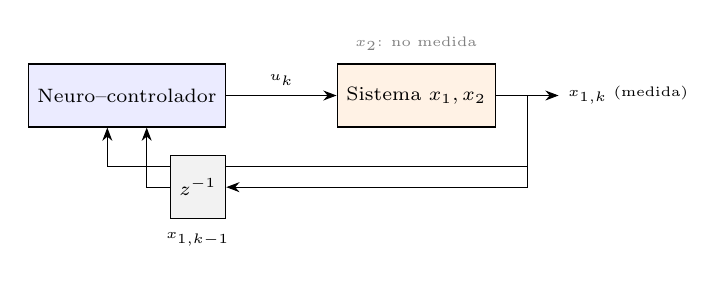
\begin{tikzpicture}[block/.style={draw,minimum height=8mm,minimum width=16mm,font=\scriptsize},
                    node distance=6mm and 10mm]
\node[block,fill=blue!8] (ctl) {Neuro--controlador};
\node[block,right=14mm of ctl,fill=orange!10] (sys) {Sistema $x_1,x_2$};
\draw[-{Stealth}] (ctl) -- node[above,font=\tiny] {$u_k$} (sys);
\draw[-{Stealth}] (sys.east) -- ++(8mm,0) node[right,font=\tiny] {$x_{1,k}$ (medida)};
\draw[-{Stealth}] ($(sys.east)+(4mm,0)$) |- ++(0,-9mm) -| ($(ctl.south)+(-2.5mm,0)$);
\node[block,minimum width=7mm,below=3.5mm of ctl,xshift=9mm,fill=gray!10] (z) {$z^{-1}$};
\draw[-{Stealth}] ($(sys.east)+(4mm,0)$) |- (z.east);
\draw[-{Stealth}] (z.west) -| ($(ctl.south)+(2.5mm,0)$);
\node[font=\tiny,below=0.5mm of z] {$x_{1,k-1}$};
\node[font=\tiny,gray] at ($(sys.north)+(0,2.5mm)$) {$x_2$: no medida};
\end{tikzpicture}
\caption{Controlador con realimentación parcial: la variable medida y sus valores pasados como entradas.}
\end{figure}

\subsection*{(b) Aprendizaje incremental para un sistema bilineal inestable en amplio rango}

Al igual que los seres humanos, la red debe entrenarse \emph{empezando con tareas simples} y continuar con tareas más complejas de manera incremental. Para la mayoría de los sistemas, las tareas simples son las cercanas a un estado estable (de equilibrio). El procedimiento:

\begin{enumerate}[itemsep=2pt]
\item \textbf{Etapa inicial (tarea simple).} Se entrena el neuro--controlador con condiciones iniciales \emph{cercanas al estado de equilibrio} $x^{*}$ (y, si conviene, horizontes de simulación $N$ cortos). Como el sistema es inestable, empezar cerca del equilibrio evita que las trayectorias diverjan durante las primeras épocas, cuando la red aún no controla, y que los gradientes crezcan descontroladamente.
\item \textbf{Ampliación progresiva.} Una vez que el costo converge, se amplía gradualmente el rango de condiciones iniciales (más lejos del equilibrio) y/o el horizonte $N$, \emph{re-usando los pesos ya entrenados como inicialización} de la nueva etapa (la red no empieza de cero: refina lo aprendido).
\item \textbf{Conjunto de posiciones iniciales.} En cada etapa se entrena simultáneamente con un \emph{conjunto} de posiciones iniciales representativas (en los programas del curso, cuatro), acumulando los gradientes de todas las trayectorias antes de actualizar los pesos; así el controlador generaliza a otras posiciones no vistas.
\item \textbf{Repetición.} Se repite el proceso hasta cubrir todo el amplio rango de operación requerido, monitoreando que el costo decrezca en cada etapa.
\end{enumerate}

\subsection*{(c) Cambios para que $\mathbf x$ converja en $\mathbf x^{*}$ (regulación / tracking)}

El neuro--controlador entrenado para estabilización ($\mathbf x\to 0$ con $u\to 0$), representado por $u_k=N(\mathbf x_k)$, se adapta cambiando \emph{apropiadamente sus entradas y su salida}:
\begin{equation}
\boxed{\;u_k = u^{*} + N(\mathbf x_k-\mathbf x^{*})\;}
\end{equation}
es decir: (i) a las entradas de la red se les resta el estado deseado $\mathbf x^{*}$ (la red ve el \emph{error} $\mathbf x_k-\mathbf x^{*}$, que debe converger a cero), y (ii) a la salida de la red se le suma el control de equilibrio $u^{*}$. Los valores $\mathbf x^{*}$ y $u^{*}$ no pueden elegirse de forma independiente: deben cumplir la \textbf{condición de equilibrio} del sistema
\begin{equation}
\mathbf x^{*}=f(\mathbf x^{*},u^{*})
\end{equation}
(para el sistema bilineal de la parte (b), esta condición determina el $u^{*}$ correspondiente a cada $\mathbf x^{*}$ alcanzable). Si se prefiere, alternativamente puede re--entrenarse la red directamente con la función de costo $J=\frac12\sum_k(\mathbf x_k-\mathbf x^{*})^{T}(\mathbf x_k-\mathbf x^{*})$, con \texttt{out\_des} $=\mathbf x^{*}$, pero la adaptación de entradas/salida evita el re--entrenamiento y permite cambiar $\mathbf x^{*}$ en línea.

%=====================================================================
\clearpage
\section*{Pregunta 5 (4 ptos) — Explicación del programa Matlab de cálculo y acumulación de derivadas totales (DBP) para el robot tipo carro}

\begin{enunciado}
Explicar el significado de cada línea del programa. Explicar cómo está implementada la ecuación recursiva del cálculo de derivadas totales según el algoritmo DBP. La posición final deseada es $y^{*}=0$, $\phi^{*}=0$; la variable \texttt{x(1,1)} corresponde a una de las coordenadas y \texttt{x(2,1)} al ángulo $\phi$. Indicar todas las matrices que deben inicializarse antes del bucle \texttt{for--end}.
\end{enunciado}

Según lo visto en la Pregunta 3, \texttt{x(1,1)}$\,=y_k$ (la coordenada que aparece en el objetivo $y^{*}=0$; en el modelo actualizado con $\sin$ de \texttt{x(2,1)}) y \texttt{x(2,1)}$\,=\phi_k$. La red tiene una capa oculta de $n_h$ neuronas sigmoideas bipolares con pesos de entrada \texttt{v}, centros \texttt{c}, pendientes \texttt{a} y pesos de salida \texttt{w}; \texttt{r}$\,=\Delta r=v\Delta t$, \texttt{L}$\,=L$, y \texttt{j} indexa la posición inicial de la trayectoria simulada (bucle externo no mostrado).

\begin{lstlisting}
for k = 1:ndata-1
   in_red = [ x(1,1)
              x(2,1) ];
   m = v'*in_red;
   n = 2.0./(1 + exp(-(m-c)./a)) - 1;
   out_red = w'*n;
   u(k,j) = out_red';
   estado(k,:,j) = x';
   jacob = [ 1  r*cos(x(2,1))
             0  1 ];
   dxdu = [ 0
            -r/L ];
   z(1,1) = x(1,1) + r*sin(x(2,1));
   z(2,1) = x(2,1) - r/L*u(k,j);
   x = z;
   dndm = diag((1 - n.*n)./(2*a));
   dudw_s = [ n ];
   dudv_s = in_red*w'*dndm;
   dudc_s = w .* ((n.*n-1)./(2.0.*a));
   duda_s = w .* ((n.*n-1).*(m-c)./(2*a.*a));
   dudx = w'*dndm*v';
   jacob_t = dxdu*dudx + jacob;
   dx1dw_t = dxdu(1,1).*dudw_s + jacob_t(1,1).*dx1dw_t + jacob_t(1,2).*dx2dw_t;
   dx2dw_t = dxdu(2,1).*dudw_s + jacob_t(2,1).*dx1dw_t + jacob_t(2,2).*dx2dw_t;
   dx1dv_t = dxdu(1,1).*dudv_s + jacob_t(1,1).*dx1dv_t + jacob_t(1,2).*dx2dv_t;
   dx2dv_t = dxdu(2,1).*dudv_s + jacob_t(2,1).*dx1dv_t + jacob_t(2,2).*dx2dv_t;
   dx1dc_t = dxdu(1,1).*dudc_s + jacob_t(1,1).*dx1dc_t + jacob_t(1,2).*dx2dc_t;
   dx2dc_t = dxdu(2,1).*dudc_s + jacob_t(2,1).*dx1dc_t + jacob_t(2,2).*dx2dc_t;
   dx1da_t = dxdu(1,1).*duda_s + jacob_t(1,1).*dx1da_t + jacob_t(1,2).*dx2da_t;
   dx2da_t = dxdu(2,1).*duda_s + jacob_t(2,1).*dx1da_t + jacob_t(2,2).*dx2da_t;
   out_des = [ 0  0 ];
   out_des = out_des';
   erJ = (x - out_des);
   dJdw_t = dJdw_t + erJ(1,1).*dx1dw_t + erJ(2,1).*dx2dw_t;
   dJdv_t = dJdv_t + erJ(1,1).*dx1dv_t + erJ(2,1).*dx2dv_t;
   dJdc_t = dJdc_t + erJ(1,1).*dx1dc_t + erJ(2,1).*dx2dc_t;
   dJda_t = dJda_t + erJ(1,1).*dx1da_t + erJ(2,1).*dx2da_t;
end
\end{lstlisting}

\subsection*{5.1 Significado de cada línea}

\textbf{Bloque A — Evaluación del neuro--controlador (líneas 1--7).}
\begin{itemize}[itemsep=1pt]
\item L1: bucle sobre los pasos de tiempo de la trayectoria simulada ($k=1,\dots,N-1$).
\item L2--3: \texttt{in\_red} es el vector de entrada de la red $=$ estado actual $[y_k;\ \phi_k]$.
\item L4: \texttt{m}$\,=v^{T}\mathbf x_k$: entradas netas (sumas ponderadas) de las neuronas ocultas.
\item L5: \texttt{n}: salidas de las neuronas ocultas con sigmoide bipolar $n_j=\frac{2}{1+e^{-(m_j-c_j)/a_j}}-1$ (rango $(-1,1)$, centro $c_j$, pendiente $a_j$).
\item L6: \texttt{out\_red}$\,=w^{T}\mathbf n$: salida de la red $=$ señal de control $u_k$.
\item L7: se almacena el control aplicado en el paso $k$ de la trayectoria $j$.
\item L8: se almacena la trayectoria del estado (para graficar/validar).
\end{itemize}

\textbf{Bloque B — Modelo del sistema y sus derivadas (líneas 9--15).}
\begin{itemize}[itemsep=1pt]
\item L9--10: \texttt{jacob}$\,=\pd{\mathbf x_{k+1}}{\mathbf x_k}=\begin{bmatrix}1 & \Delta r\cos\phi_k\\ 0 & 1\end{bmatrix}$: Jacobiano del modelo discretizado del robot (término que aporta \emph{el modelo del sistema} a la ecuación recursiva).
\item L11--12: \texttt{dxdu}$\,=\pd{\mathbf x_{k+1}}{u_k}=[\,0;\ -\Delta r/L\,]$: sensibilidad del estado siguiente respecto al control (también del \emph{modelo}).
\item L13--14: ecuaciones de movimiento discretizadas: $y_{k+1}=y_k+\Delta r\sin\phi_k$;\quad $\phi_{k+1}=\phi_k-\frac{\Delta r}{L}u_k$.
\item L15: se avanza el estado: $\mathbf x_k\leftarrow\mathbf x_{k+1}$ (simulación del lazo cerrado).
\end{itemize}

\textbf{Bloque C — Derivadas simples del neuro--controlador (líneas 16--21).}
\begin{itemize}[itemsep=1pt]
\item L16: \texttt{dndm}$\,=\mathrm{diag}\bigl(\frac{1-n_j^2}{2a_j}\bigr)$: derivada de la sigmoide bipolar respecto a su entrada neta.
\item L17: \texttt{dudw\_s}$\,=\pd{u_k}{w}=\mathbf n$ (derivada \emph{simple}: sufijo \texttt{\_s}).
\item L18: \texttt{dudv\_s}$\,=\pd{u_k}{v}=\mathbf x_k\,(w^{T}D)$, matriz $2\times n_h$ con componentes $x_i\,w_j\,n_j'$.
\item L19: \texttt{dudc\_s}$\,=\pd{u_k}{c}$: como $\pd{n_j}{c_j}=-\pd{n_j}{m_j}$, resulta $w_j\frac{n_j^2-1}{2a_j}$.
\item L20: \texttt{duda\_s}$\,=\pd{u_k}{a}=w_j\frac{(n_j^2-1)(m_j-c_j)}{2a_j^2}$.
\item L21: \texttt{dudx}$\,=\pd{u_k}{\mathbf x_k}=w^{T}Dv^{T}=[\,\pd{u}{y}\ \ \pd{u}{\phi}\,]$: sensibilidad del control respecto al estado (del \emph{neuro--controlador}).
\end{itemize}

\textbf{Bloque D — Ecuación recursiva del DBP (líneas 22--30).}
\begin{itemize}[itemsep=1pt]
\item L22: \texttt{jacob\_t}$\,=$ \texttt{dxdu*dudx + jacob} $=\pd{\mathbf x_{k+1}}{u_k}\pd{u_k}{\mathbf x_k}+\pd{\mathbf x_{k+1}}{\mathbf x_k}=J_t$: \textbf{Jacobiano del lazo cerrado} (combina modelo y controlador).
\item L23--30: implementan, componente a componente y para cada grupo de parámetros $\theta\in\{w,v,c,a\}$, la ecuación recursiva
\[
\td{\mathbf x_{k+1}}{\theta}=\pd{\mathbf x_{k+1}}{u_k}\pd{u_k}{\theta}+J_t\,\td{\mathbf x_k}{\theta}
\]
La fila 1 (variable $y$): \texttt{dx1d}$\theta$\texttt{\_t}$\,=$\texttt{dxdu(1,1)}$\cdot\pd{u}{\theta}+J_t(1,1)\,$\texttt{dx1d}$\theta$\texttt{\_t}$+J_t(1,2)\,$\texttt{dx2d}$\theta$\texttt{\_t}, y análogamente la fila 2 (variable $\phi$). En el lado derecho, \texttt{dx1d}$\theta$\texttt{\_t} y \texttt{dx2d}$\theta$\texttt{\_t} contienen los valores del paso \emph{anterior} ($\td{\mathbf x_k}{\theta}$), y tras la asignación quedan actualizadas al paso $k+1$.
\end{itemize}

\textbf{Bloque E — Error y acumulación del gradiente del costo (líneas 31--38).}
\begin{itemize}[itemsep=1pt]
\item L31--32: \texttt{out\_des}$\,=[y^{*};\ \phi^{*}]=[0;0]$: posición final deseada.
\item L33: \texttt{erJ}$\,=\mathbf x_{k+1}-\mathbf x^{*}$: error de la trayectoria en el paso $k+1$ (nótese que \texttt{x} ya fue actualizado en L15, coherente con que las derivadas totales calculadas corresponden a $\mathbf x_{k+1}$).
\item L34--37: acumulación del gradiente total del costo $J=\frac12\sum_k\|\mathbf x_k-\mathbf x^{*}\|^2$:
\[
\td{J}{\theta}\ \mathrel{+}=\ (\mathbf x_{k+1}-\mathbf x^{*})^{T}\,\td{\mathbf x_{k+1}}{\theta}
= e_1\,\texttt{dx1d}\theta\texttt{\_t}+e_2\,\texttt{dx2d}\theta\texttt{\_t}
\]
Al terminar el bucle, \texttt{dJdw\_t}, \texttt{dJdv\_t}, \texttt{dJdc\_t}, \texttt{dJda\_t} contienen los gradientes totales listos para actualizar los pesos por gradiente descendente ($w\leftarrow w-\eta\,\texttt{dJdw\_t}$, etc., típicamente tras acumular sobre todas las posiciones iniciales $j$).
\end{itemize}

\subsection*{5.2 Cómo está implementada la ecuación recursiva del DBP}

La ecuación recursiva \eqref{eq:dbp} aparece en el programa en dos partes:
\begin{enumerate}[itemsep=2pt]
\item \textbf{Construcción del Jacobiano de lazo cerrado} (L22): \texttt{jacob\_t = dxdu*dudx + jacob}, que corresponde exactamente al término entre corchetes de \eqref{eq:dbp}: la matriz $2\times2$ que propaga las derivadas totales del paso $k$ al paso $k+1$; combina el \emph{modelo} (\texttt{jacob}, \texttt{dxdu}) con el \emph{controlador} (\texttt{dudx}).
\item \textbf{Propagación + inyección} (L23--30): cada línea suma (i) el \textbf{aporte nuevo} del paso presente, $\pd{\mathbf x_{k+1}}{u_k}\pd{u_k}{\theta}$ (producto \texttt{dxdu(i,1)}$\times$derivada simple \texttt{dud}$\theta$\texttt{\_s}), con (ii) la \textbf{propagación} de la historia acumulada, $J_t\,\td{\mathbf x_k}{\theta}$ (combinación de \texttt{dx1d}$\theta$\texttt{\_t} y \texttt{dx2d}$\theta$\texttt{\_t} del paso anterior con los elementos de \texttt{jacob\_t}). La recursión se inicializa en cero antes del bucle y avanza \emph{hacia adelante} junto con la simulación: por eso el DBP no necesita almacenar toda la trayectoria como el BPTT.
\end{enumerate}

\emph{Observación fina:} en rigor, las dos filas de cada grupo deberían actualizarse \emph{simultáneamente} (la línea de \texttt{dx2dw\_t} usa \texttt{dx1dw\_t} que acaba de ser sobrescrito); una implementación estricta guarda copias temporales de los valores del paso anterior antes de actualizar. El efecto numérico es pequeño si $\Delta r$ es pequeño (los términos cruzados son de orden $\Delta r$), pero es un detalle a cuidar al programar.

\subsection*{5.3 Matrices que deben inicializarse antes del bucle \texttt{for--end}}

Con $n_h$ el número de neuronas ocultas:

\begin{center}
\renewcommand{\arraystretch}{1.3}
\small
\begin{tabular}{l l l}
\toprule
Variable & Dimensión & Inicialización\\
\midrule
\texttt{x} & $2\times1$ & posición inicial $[y_0;\ \phi_0]$ de la trayectoria $j$\\
\texttt{v} & $2\times n_h$ & pesos de entrada de la red (aleatorios pequeños)\\
\texttt{c}, \texttt{a}, \texttt{w} & $n_h\times1$ c/u & centros, pendientes y pesos de salida de la red\\
\texttt{dx1dw\_t}, \texttt{dx2dw\_t} & $n_h\times1$ & \textbf{ceros} (condición inicial $\td{\mathbf x_0}{w}=0$)\\
\texttt{dx1dv\_t}, \texttt{dx2dv\_t} & $2\times n_h$ & \textbf{ceros}\\
\texttt{dx1dc\_t}, \texttt{dx2dc\_t} & $n_h\times1$ & \textbf{ceros}\\
\texttt{dx1da\_t}, \texttt{dx2da\_t} & $n_h\times1$ & \textbf{ceros}\\
\texttt{dJdw\_t} & $n_h\times1$ & \textbf{ceros}\\
\texttt{dJdv\_t} & $2\times n_h$ & \textbf{ceros}\\
\texttt{dJdc\_t}, \texttt{dJda\_t} & $n_h\times1$ & \textbf{ceros}\\
\texttt{u}, \texttt{estado}, \texttt{z} & --- & arreglos de almacenamiento (y \texttt{z} $2\times1$)\\
\texttt{r}, \texttt{L}, \texttt{ndata} & escalares & $\Delta r=v\Delta t$, longitud del robot, número de datos\\
\bottomrule
\end{tabular}
\end{center}

\textbf{Precisión importante sobre el alcance de la inicialización:} las derivadas totales de estado (\texttt{dx1d}$\theta$\texttt{\_t}, \texttt{dx2d}$\theta$\texttt{\_t}) deben ponerse en cero \emph{al inicio de cada trayectoria} (cada posición inicial $j$), porque cada trayectoria comienza con un estado inicial que no depende de los pesos. En cambio, los acumuladores del gradiente (\texttt{dJdw\_t}, \texttt{dJdv\_t}, \texttt{dJdc\_t}, \texttt{dJda\_t}) se ponen en cero \emph{una vez por época de entrenamiento}, antes del bucle sobre las posiciones iniciales, porque acumulan el gradiente sobre todos los pasos $k$ \emph{y} todas las trayectorias $j$ (aprendizaje tipo batch con varias posiciones iniciales, como se indicó en la Pregunta 4(b)).

\vspace{16pt}
\begin{center}
\small\itshape Lima, julio de 2026 --- Documento de estudio basado íntegramente en el material del curso.
\end{center}

\end{document}
